\begin{frame}{¿Por qué un laboratorio remoto?}
\begin{itemize}
    \item Reducir riesgos
    \begin{itemize}
        \item Pandemias.
        \item Uso de materiales peligrosos.
    \end{itemize}
    \item Una pieza más en educación remota.
    \item Reducir barreras de acceso
    \begin{itemize}
        \item Geográficas.
        \item Económicas.
        \item Culturales.
    \end{itemize}
    \item Aumentar el uso de equipos.
    \begin{itemize}
        \item Amortizar inversión.
    \end{itemize}
\end{itemize}
\end{frame}

\begin{frame}{Fases de desarrollo de un laboratorio remoto}
\begin{itemize}
    \item El desarrollo no sigue una secuencia fija.
    \begin{itemize}
        \item Laboratorio Virtual. Simulación. No se experimentó
        \item Acceso a Datos Reales. Descargar registros sincrónicos o un conjunto de datos. Se usó en la cohorte 2021
        \item Control Remoto. Los estudiantes controlan efectivamente un sistema y registran las medidas. Se usa en 2022 y 2023.
        \item Plus: Elementos robóticos a distancia. Se inicia en 2023.
    \end{itemize}
\end{itemize}
\end{frame}

\begin{frame}{Laboratorio remoto}
\begin{columns}[c] % The "c" option specifies centered vertical alignment while the "t" option is used for top vertical alignment

\column{.58\textwidth}
\begin{itemize}
	\item Nuestro laboratorio cumple con los estándares de un laboratorio remoto.
    \item El modelo está organizado en tres capas.
    \begin{itemize}
        \item Laboratorio Físico.
        \item Ecosistema de Comunicación.
        \item Contenidos.
    \end{itemize}

\end{itemize}
\column{.38\textwidth} % Right column and width

\begin{tikzpicture}[->,>=stealth',square/.style={regular polygon,regular polygon sides=4},hex/.style={regular polygon,regular polygon sides=6, minimum size = 3cm},scale=0.3, every node/.style={scale=0.3}]
        \node at (-3.118,1.8) [hex,draw] (conf) {Reg};
        %\node at (-3.118,-1.8) [hex,draw] (cat) {Chat};
        \node at (0,-3.6) [hex,draw] (documentosVersiones) {Docs};
        %\node at (3.118,-1.8) [hex,draw] (data) {Data};
        \node at (3.118,1.8) [hex,draw] (app) {APP};
        %\node at (0,3.6) [hex,draw] (compu) {Cloud C};
        
        \node at (0,0) [circle,draw,minimum size = 3.5cm] (lab) {LAB};
        
        \node[isosceles triangle,
        	isosceles triangle apex angle=50,
    		draw,
    		rotate=-30,
    		%fill=teal!30,
    		minimum size =0.866cm] (T30)at (-4.936,2.85){};
    	
    	\node[draw,text width=2.2cm] at (-6.928,4) {Student registration for practices. Publication of calendars. Report submission. Access to restricted areas.};
    	
    	%\begin{comment}	
    	%\node[isosceles triangle,
        %	isosceles triangle apex angle=50,
    	%	draw,
    	%	rotate=-60,
    	%	%fill=teal!30,
    	%	minimum size =0.866cm] (T30)at (-4.936,-2.85){};
    	%	
    	%\node[draw,text width=2.2cm] at (-6.928,-4) {Restricted messaging channel for staff and students.};
    	%\end{comment}
    	
    	\node[isosceles triangle,
        	isosceles triangle apex angle=50,
    		draw,
    		rotate=0,
    		%fill=teal!30,
    		minimum size =0.866cm] (T30)at (0,-5.7){};
    		
    	\node[draw,text width=4cm] at (0,-8) {Documentation service: Public information about the practice topic. Restricted access to codes and space to store practice products.};
    		
    	%\node[isosceles triangle,
        %	isosceles triangle apex angle=50,
    	%	draw,
    	%	rotate=60,
    	%	%fill=teal!30,
    	%	minimum size =0.866cm] (T30)at (4.936,-2.85){};
    	%	
    	%\node[draw,text width=2.2cm] at (6.928,-4) {Restricted data repository and space to store and access collected data (optional).};
    		
    	\node[isosceles triangle,
        	isosceles triangle apex angle=50,
    		draw,
    		rotate=120,
    		%fill=teal!30,
    		minimum size =0.866cm] (T30)at (4.936,2.85){};
    		
    	\node[draw,text width=2.2cm] at (6.928,4) {Access control to the remote laboratory according to the schedule. Virtual lab. Instrument management. Data collection. Video, Augmented Reality, etc.};
    		
    	%\node[isosceles triangle,
        %	isosceles triangle apex angle=50,
    	%	draw,
    	%	rotate=90,
    	%	%fill=teal!30,
    	%	minimum size =0.866cm] (T30)at (0,5.7){};
        %
        %\node at (0,8) [square,draw] (compu3) {Report};
        %\node[draw,text width=4cm] at (0,8) {Final product: report, data, and codes generated by students. Delivered on the platform.};
        
    \end{tikzpicture}


\end{columns}
\end{frame}

\begin{frame}{Laboratorio físico}
\begin{itemize}
    \item Ubicado en espacio dedicado.
    \item Gestionado por software de control.
    \begin{itemize}
    	\item Equipamiento debe ser accesible mediante una GUI de monitoreo y control.
    	\item Implica hardware I/O, ADC, etc.
	\end{itemize}
    \item Requiere internet estable en ambos extremos (recomendado > 5 Mbps, < 100 ms de latencia).
\end{itemize}
\end{frame}

\begin{frame}{Ecosistema de Comunicación}
\begin{itemize}
    \item Facilita interacción entre docentes y estudiantes.
    \item Incluye gestión, documentación y acceso al laboratorio.
    \item MiLab: Mensajería, repositorio, nube.
\end{itemize}
\begin{center}
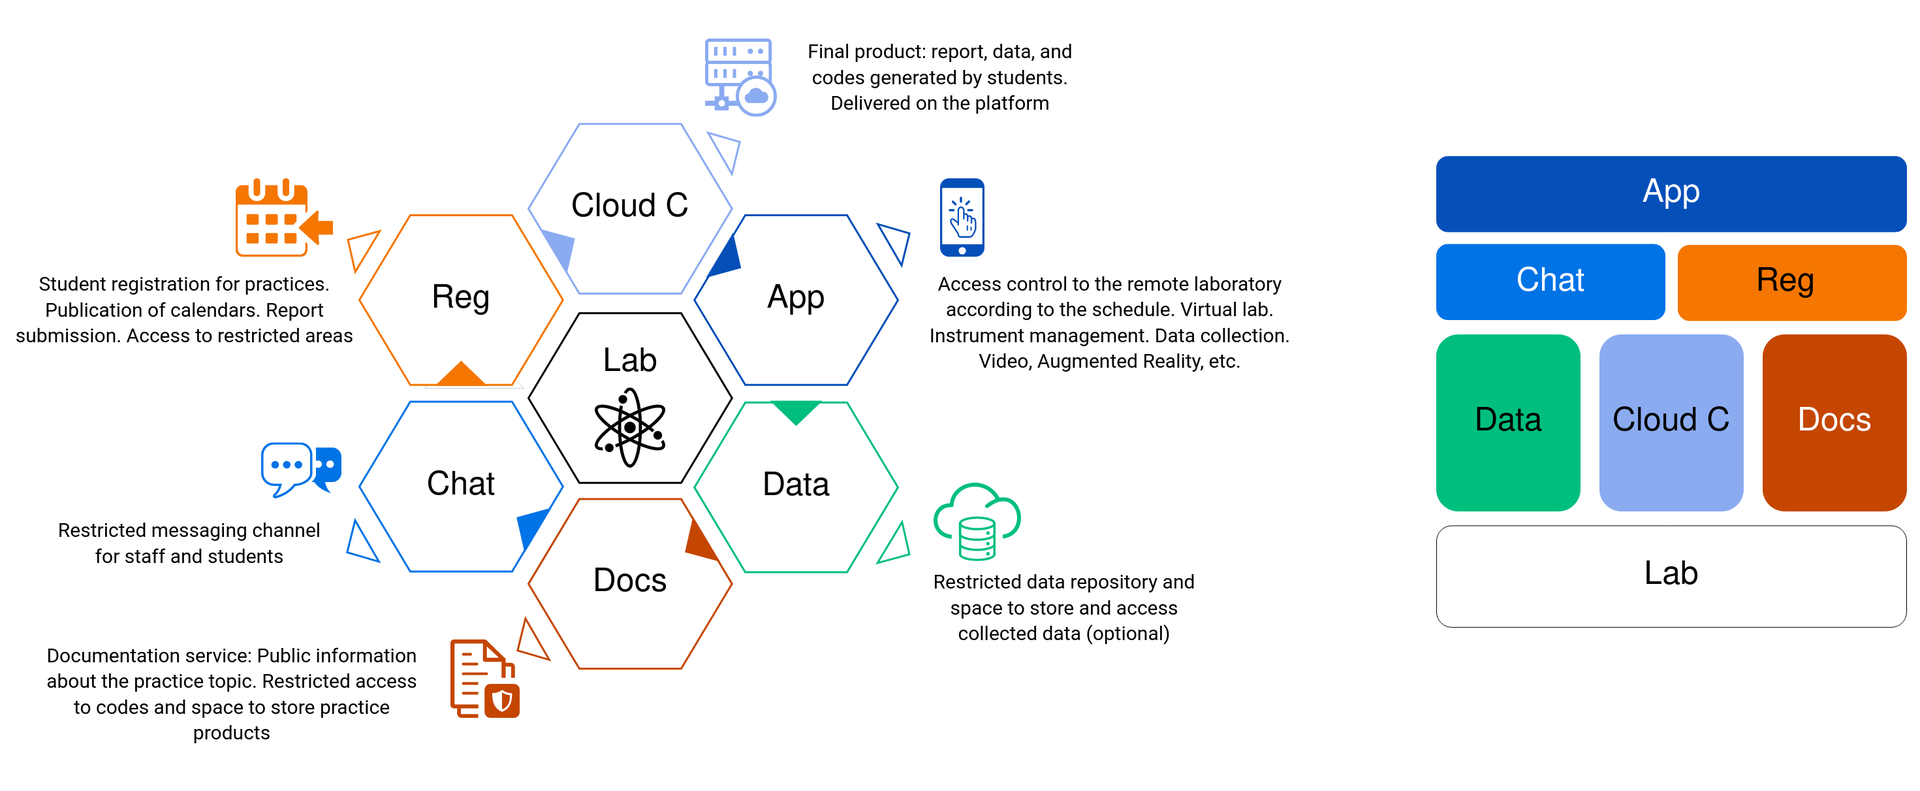
\includegraphics[scale=0.15]{imagenes/remotelabs.png}
\end{center}
\end{frame}

\begin{frame}{Contenido}
\begin{itemize}
    \item Generación por personal (guías, planes).
    \item Diseño curricular.
    \item Generación por estudiantes (datos, informes).
\end{itemize}
\end{frame}

\begin{frame}{Prácticas: Caracterización de Fotomultiplicadores}
Determinar parámetros de operación óptimos.

\begin{center}
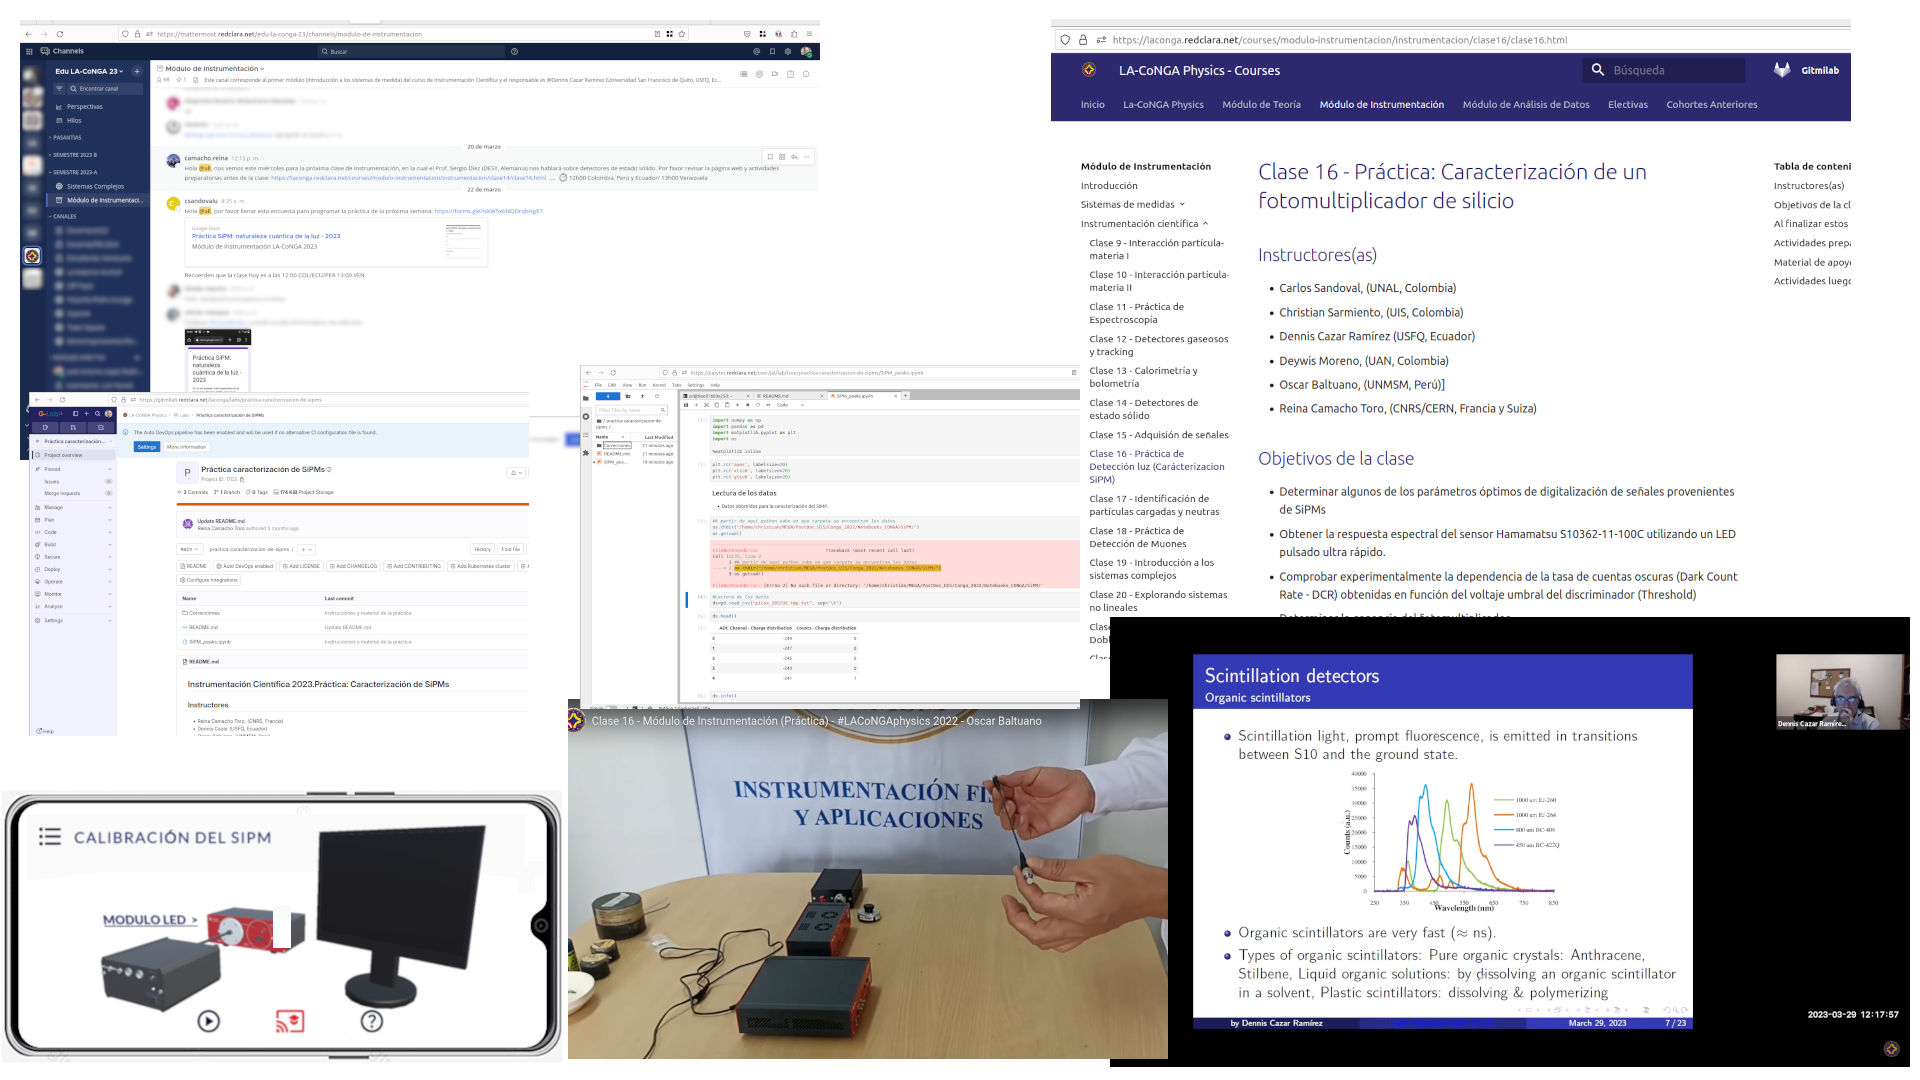
\includegraphics[scale=0.6]{imagenes/SiPM-WF.png}
\end{center}
\end{frame}

\begin{frame}{Prácticas: Espectroscopía de Fotones}
Comprender procesos radiactivos y detección de fotones.
\begin{center}
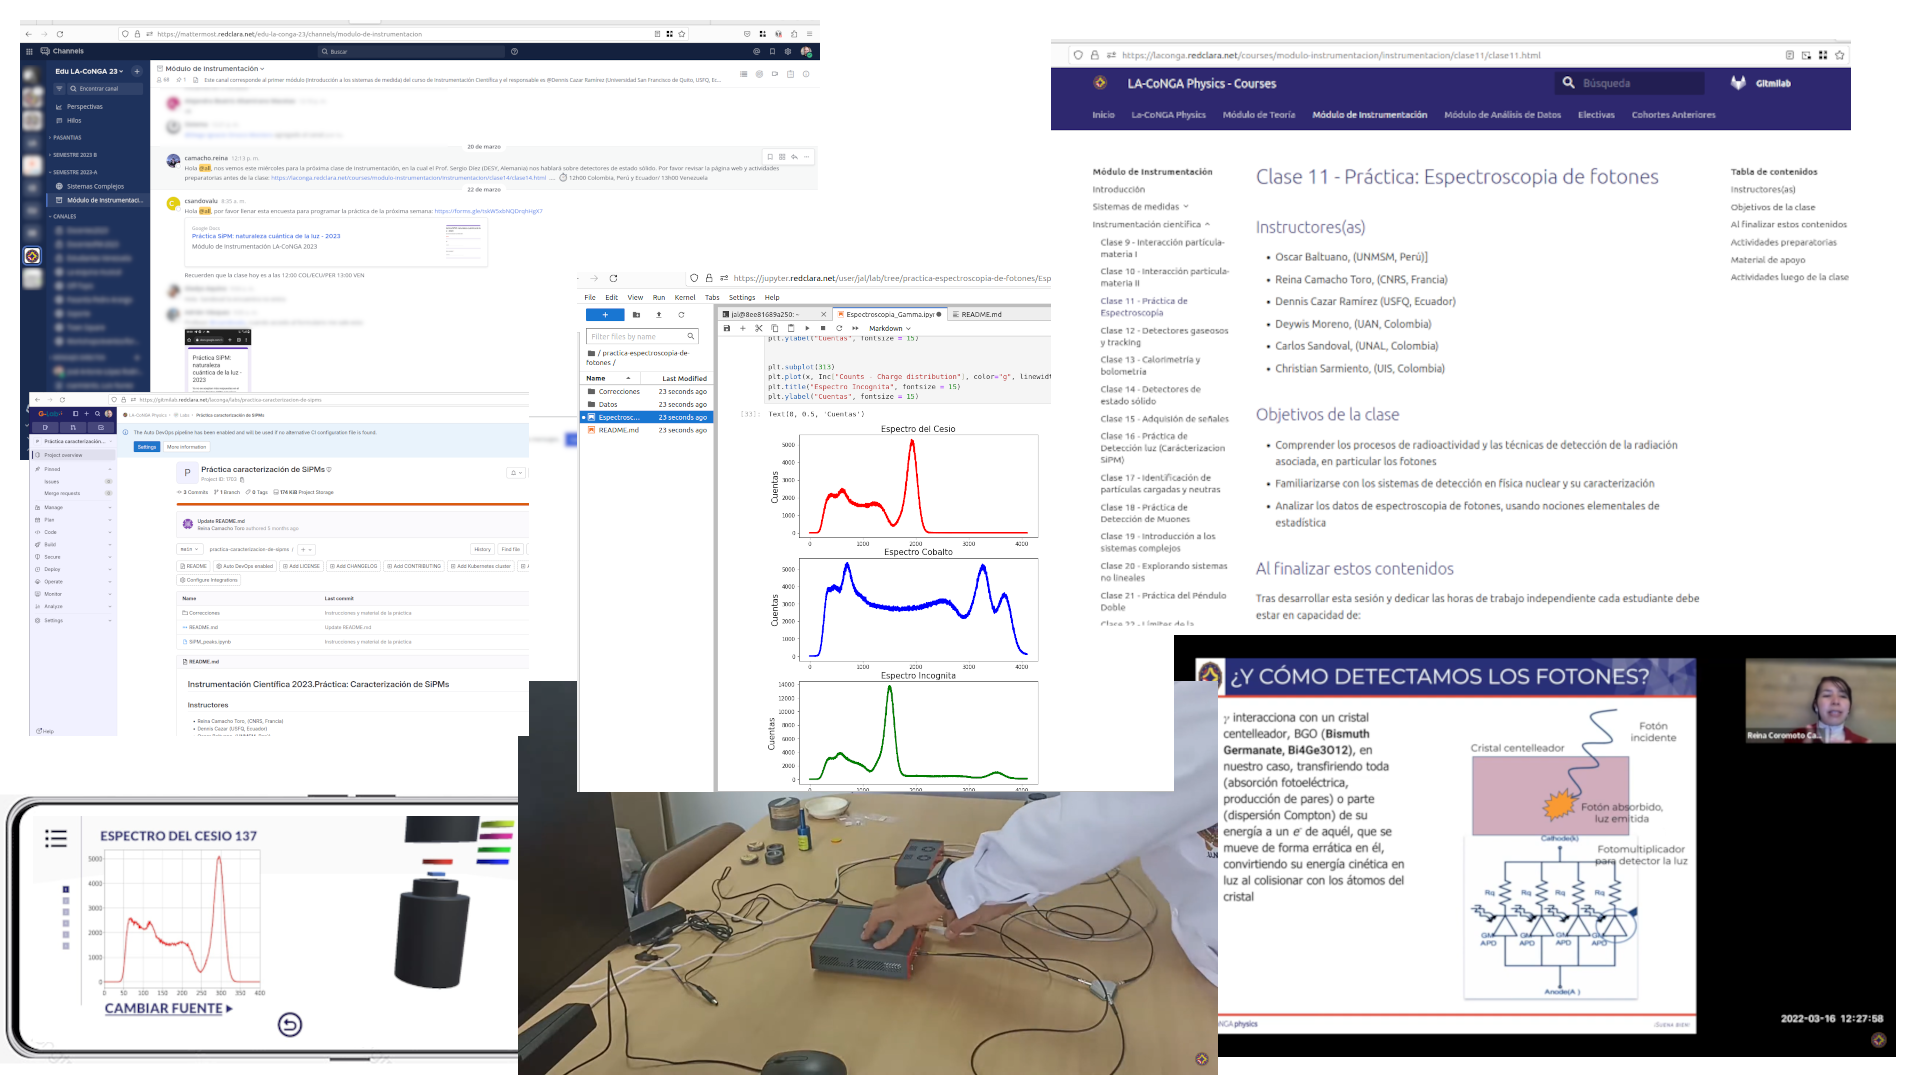
\includegraphics[scale=0.6]{imagenes/gamma-WF.png}
\end{center}
\end{frame}


\begin{frame}{Prácticas: Detección de Muones Cósmicos}
Detectar flujo de muones en distintos ángulos.
\begin{center}
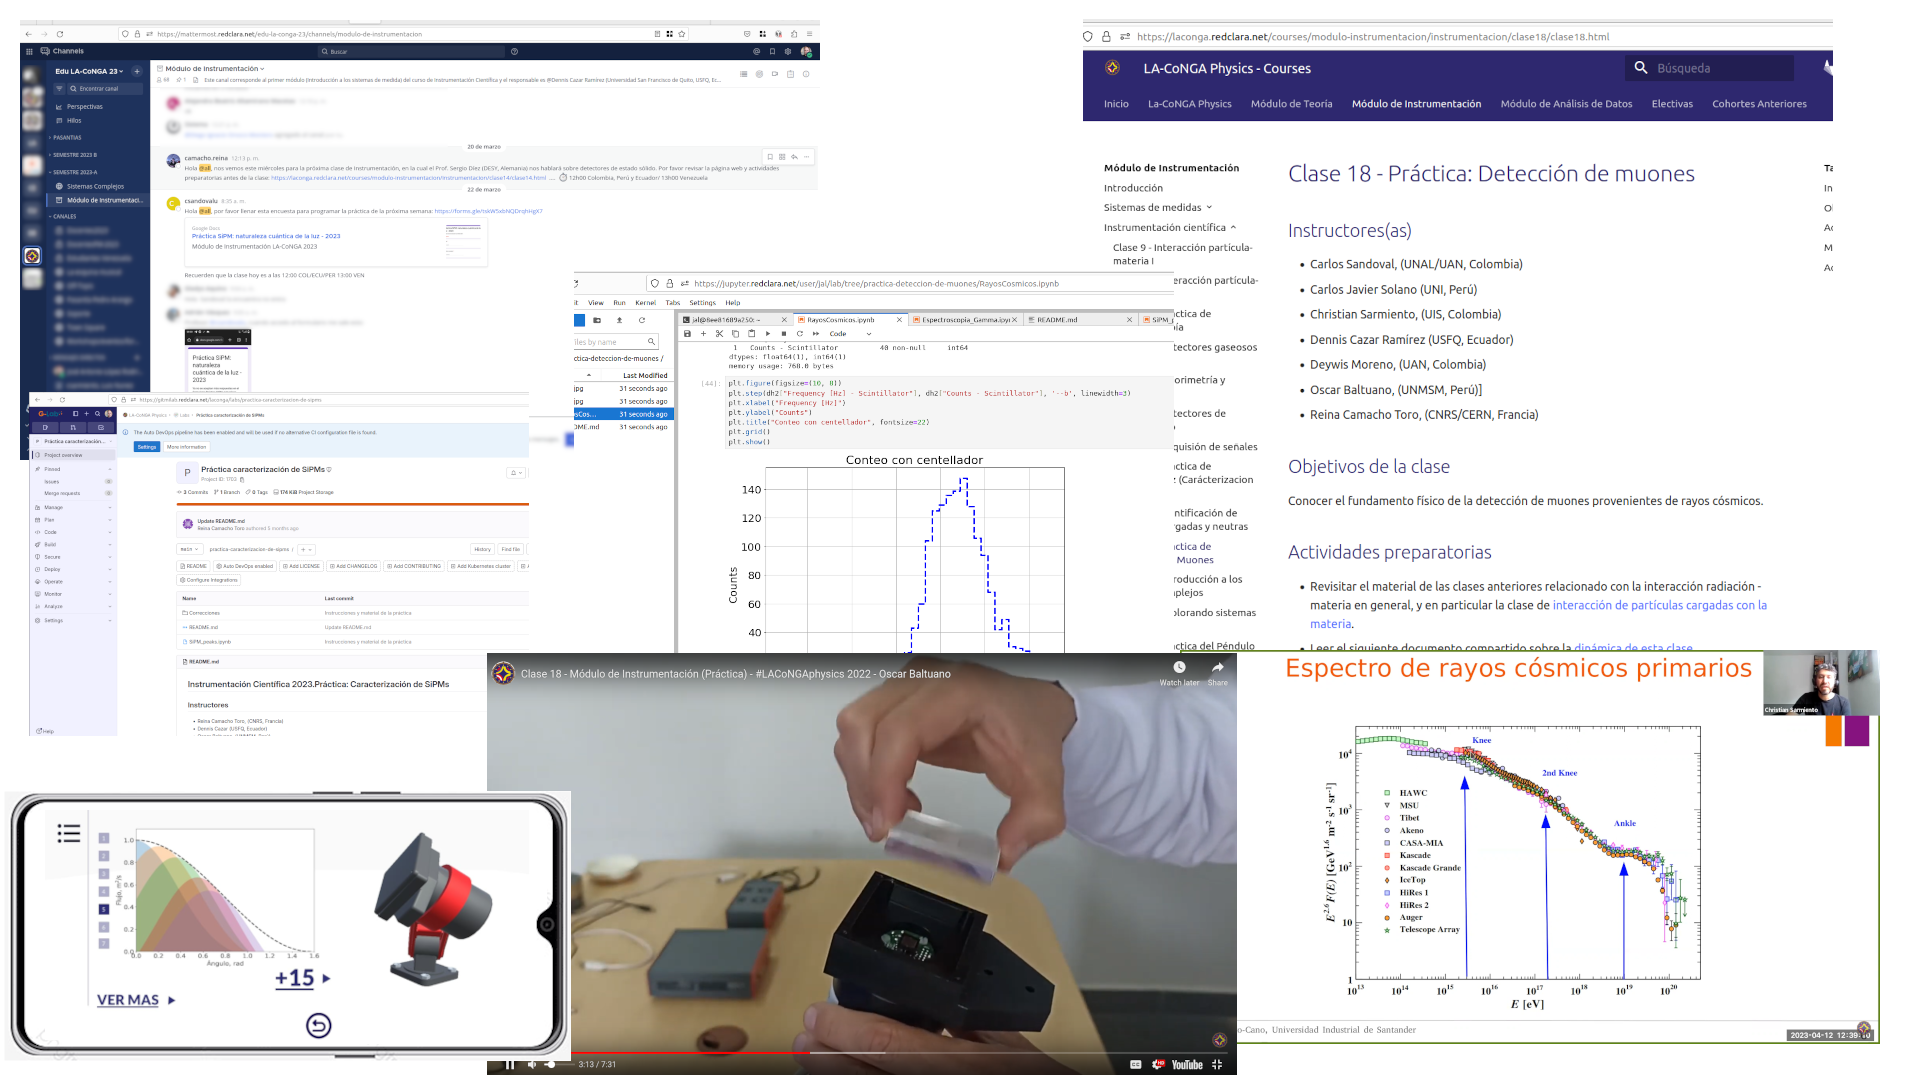
\includegraphics[scale=0.6]{imagenes/muon-WF.png}
\end{center}
\end{frame}

\begin{frame}{Prácticas: Péndulo Doble}
Estudiar sistemas caóticos.
\begin{center}
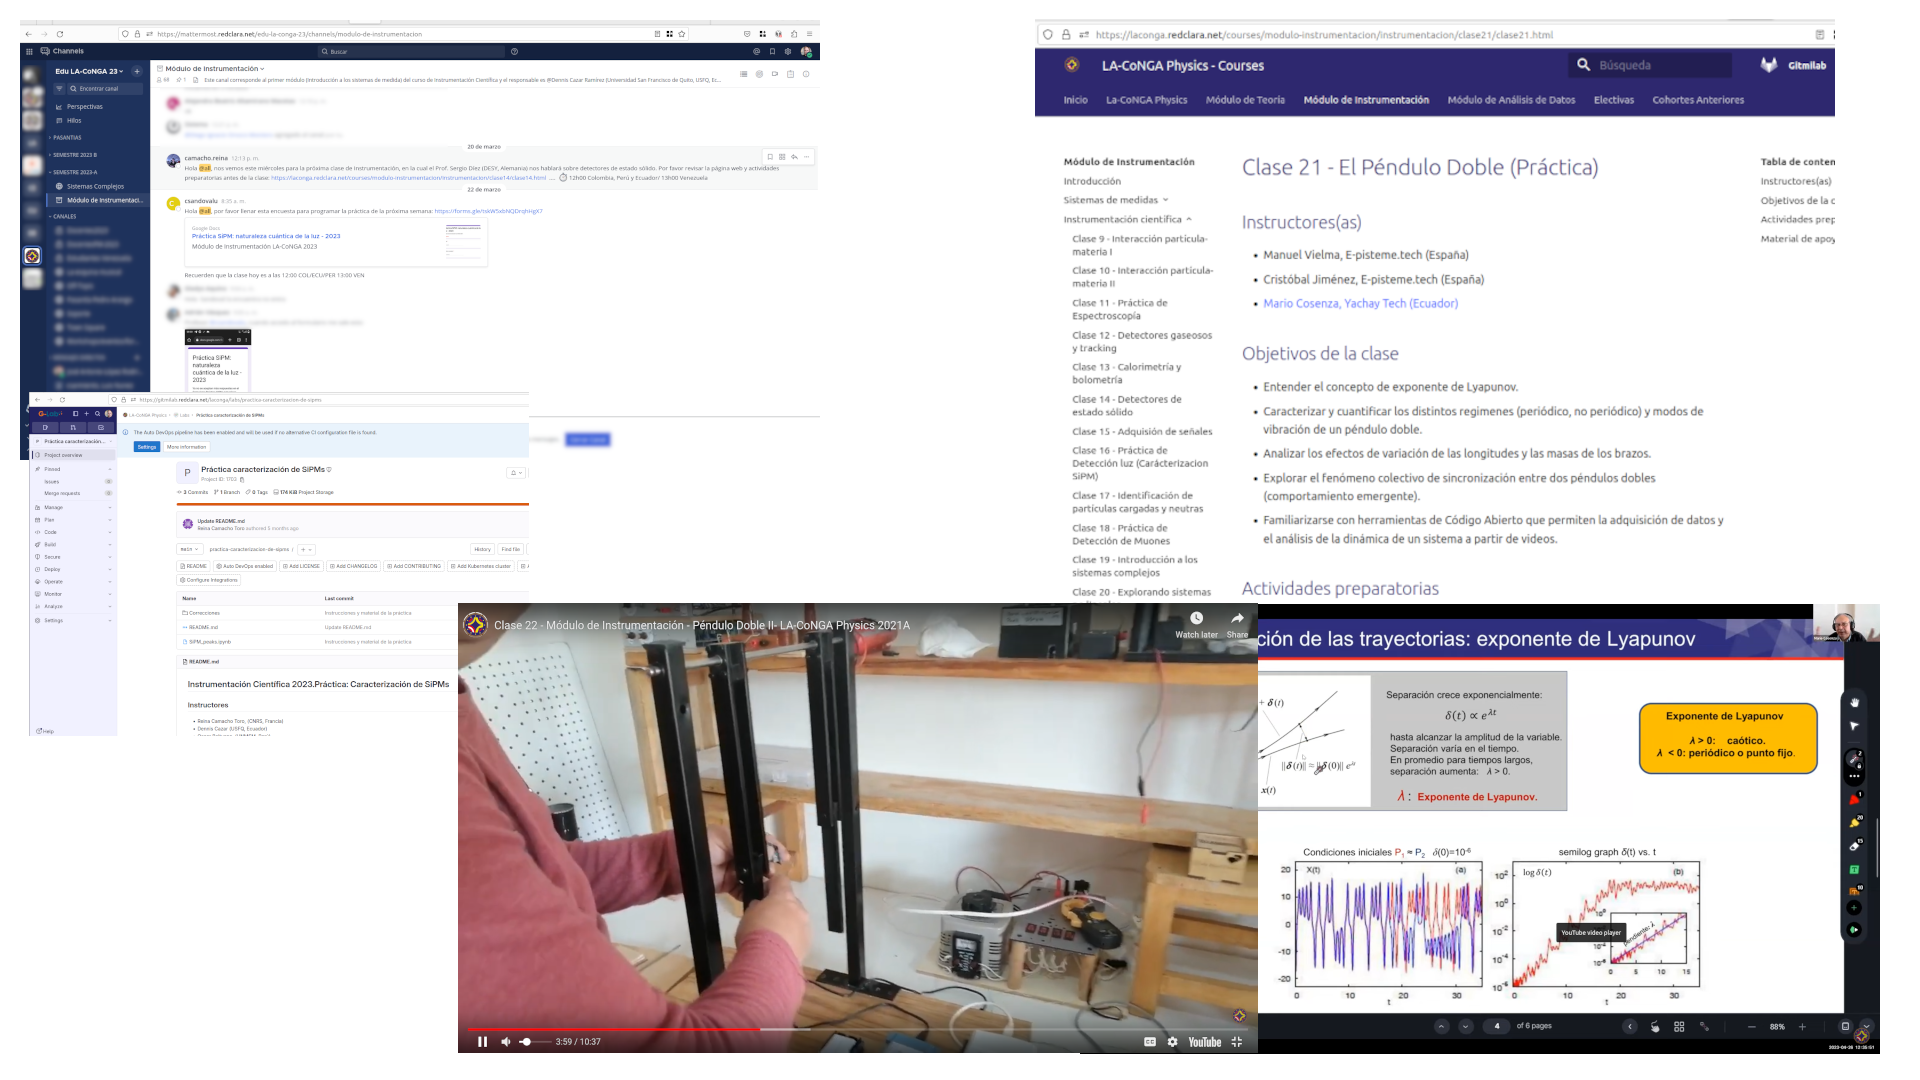
\includegraphics[scale=0.6]{imagenes/penduloDoble-WF.png}
\end{center}
\end{frame}

\begin{frame}{Resultados}
Parte del curso de Instrumentación en LA-CoNGA physics 2022-2023, con prácticas exitosas para 27 estudiantes.
\end{frame}

\begin{frame}{Conclusiones}
\begin{itemize}
    \item Éxito en la colaboración LA-CoNGA.
    \item Acceso a experiencias, reduciendo inversión.
    \item Desarrollo de capacidades remotas y competencias técnicas.
    \item Es necesario seguir desarrollando capacidades.
\end{itemize}
\end{frame}